\documentclass[12pt]{report}
\usepackage{%
	amsfonts,%
	amsmath,%	
	amssymb,%
	amsthm,%
	algorithm,%
%	babel,%
	bbm,%
	etex,%
	%biblatex,%
	caption,%
	centernot,%
	color,%
	dsfont,%
	enumerate,%
	epsfig,%
	epstopdf,%
	geometry,%
	graphicx,%
	hyperref,%
	latexsym,%
	mathtools,%
	multicol,%
	pgf,%
	pgfplots,%
	pgfplotstable,%
	pgfpages,%
	proof,%
	psfrag,%
	subfigure,%	
	tikz,%
	ulem,%
	url%
}
\usepackage{qtree}
\usepackage[fleqn]{amsmath}
\usepackage{amsthm}
\usepackage{csquotes} 
\usepackage[noend]{algpseudocode}
\usepackage[mathscr]{eucal}
\usepgflibrary{shapes}
\usetikzlibrary{%
  	arrows,%
	backgrounds,%
	chains,%
	decorations.pathmorphing,% /pgf/decoration/random steps | erste Graphik
	decorations.text,%
	matrix,%
  	positioning,% wg. " of "
  	fit,%
	patterns,%
  	petri,%
	plotmarks,%
  	scopes,%
	shadows,%
  	shapes.misc,% wg. rounded rectangle
  	shapes.arrows,%
	shapes.callouts,%
  	shapes%
}

\theoremstyle{plain}
\newtheorem{thm}{Theorem}[section]
\newtheorem{lem}[thm]{Lemma}
\newtheorem{prop}[thm]{Proposition}
\newtheorem{cor}[thm]{Corollary}

\theoremstyle{definition}
\newtheorem{defn}[thm]{Definition}
\newtheorem{conj}[thm]{Conjecture}
\newtheorem{exmp}[thm]{Example}
\newtheorem{assum}[thm]{Assumption}
\newtheorem{axiom}[thm]{Axiom}
\newtheorem{theorem}{Theorem}[section]
\newtheorem{corollary}{Corollary}[theorem]
\newtheorem{lemma}[theorem]{Lemma}



\theoremstyle{remark}
\newtheorem{rem}{Remark}
\newtheorem{note}{Note}
\newtheorem{fact}{Fact}

\newcommand{\norm}[1]{\left\lVert#1\right\rVert}
\newcommand{\indep}{\!\perp\!\!\!\perp}
\DeclarePairedDelimiter\abs{\lvert}{\rvert}%
\newcommand\numberthis{\addtocounter{equation}{1}\tag{\theequation}}
\newcommand{\tr}{\operatorname{tr}}
\newcommand{\R}{\mathbb{R}}
\newcommand{\N}{\mathbb{N}}
\newcommand{\E}{\mathbb{E}}
\newcommand{\Z}{\mathbb{Z}}
\newcommand{\B}{\mathscr{B}}
\newcommand{\C}{\mathcal{C}}
\newcommand{\T}{\mathscr{T}}
\newcommand{\F}{\mathcal{F}}
\newcommand{\G}{\mathcal{G}}
%\newcommand{\ba}{\begin{align*}}
%\newcommand{\ea}{\end{align*}}
\newcommand{\expect}[1]{\mathbb{E}\left[{#1}\right]}
\newcommand{\prob}[1]{\mathbb{P}\left[{#1}\right]}
\newcommand{\probo}[1]{\mathbb{P}_0\left[{#1}\right]}
\newcommand{\probi}[1]{\mathbb{P}_1\left[{#1}\right]}
\newcommand{\given}{\; \big\vert \;} 
\newcommand{\bydef}{:=}
\newcommand{\indic}[1]{\mathbbm{1}\{#1\}}
\DeclareMathOperator*{\argmax}{arg\,max}
\renewcommand{\qedsymbol}{$\blacksquare$}
\makeatletter
\def\BState{\State\hskip-\ALG@thistlm}
\makeatother

\makeatletter
\def\th@plain{%
  \thm@notefont{}% same as heading font
  \itshape % body font
}
\def\th@definition{%
  \thm@notefont{}% same as heading font
  \normalfont % body font
}
\makeatother
\date{}
\usepackage{scribe_e1244}
\usepackage{times}
\begin{document}
\lecturer{Aditya Gopalan}			% optional, put lecturer's name here
\scribe{K.K.Srinivas, R.Shreyas}	% required, put your name here
\lecturenumber{8}					% required, must be a number
\lecturedate{January 31}			% required, omit year
\maketitle

% title of the lecture
\begin{center}
{\Large \bf Continuation of Composite Hypothesis Testing}
\end{center}

% ----------------------------------------------------------------------
\section{Recap}

%\subsection{Composite Hypothesis Testing}

\subsubsection{Some Notations}
\begin{itemize}
    \item $\Gamma$ : Observation Space.
    \item $\Lambda$ : Parameter Space.
    \item $\Lambda_j$ : Space of parameters corresponding to Hypothesis $H_j$.
    \item $\mathbb{P}_{\theta}$ : Probability distribution on $\Gamma$, $\theta \in \Gamma_{0}$.
    \item $\pi$ : Prior distribution on $\Lambda$.
    \item $C(i,\theta)$ : Cost of answering '$i$' when the observation came from distribution $\mathbb{P}_{\theta}$, $\theta \in \Gamma_{0}$
    \item $\delta: \Gamma \to \{0, 1\}$ : (Deterministic) Decision Rule.
    \item $\delta: \Gamma \to [0, 1]$ : (Randomized) Decision Rule (On observing $y \in \Gamma$,  $1$ is output with probability $\delta(y)$) .
    \item $R_{\theta}(\delta) \triangleq \mathbb{E}_{\theta}[C(\delta(Y),\theta)]$ : Conditional risk (Expected cost incurred when the observation came from distribution $\mathbb{P}_{\theta}$, $\theta \in \Gamma_{0}$)
    \item $r(\delta) \triangleq \mathbb{E}[C(\delta(Y),\Theta)]$ : Bayes risk.
    
\end{itemize}

\subsubsection{Bayesian Composite Hypothesis Testing}

\noindent For uniform costs, i.e,
\begin{align*}
    \Lambda = \Lambda_0 \cup \Lambda_1, \Lambda_0 \cap \Lambda_1 &= \phi \\
    C(i,\theta) = c_{ij} \forall \theta \in \Lambda_j, j &\in {0,1}    
\end{align*}

We showed that the Bayes decision rules take the form:
\begin{align*}
    \delta(y)=\begin{cases}
    1 &L(y) \geq \tau \\
    0 & \text{otherwise}
    \end{cases}
\end{align*}

where
\begin{align*}
    L(y) &= \frac{p(y|\Theta \in \Lambda_1)}{p(y|\Theta \in \Lambda_0)} \\
    \tau &= \frac{\pi_{0}(c_{00}-c_{10})}{\pi_{0}(c_{11}-c_{01})}\\
    \pi_j &\triangleq \mathbb{P}[\Theta \in \Lambda_j]
\end{align*}


\section{Neyman Pearson Composite Hypothesis Tests}

Suppose $\Lambda = \Lambda_0 \cup \Lambda_1, \Lambda_0 \cap \Lambda_1 = \phi $\\
Consider randomized decision rules $\delta: \Gamma \to [0, 1]$

\begin{defn}
The \textbf{False Alarm Probability} of $\delta$, for $\theta \in \Lambda_0$ is
\begin{equation}
    P_F(\delta,\theta) \triangleq \mathbb{E}_{\theta}[\delta(y)]
\end{equation}    


\end{defn}

\begin{defn}
The \textbf{Detection Probability} of $\delta$, for $\theta \in \Lambda_1$ is
\begin{equation}
    P_D(\delta,\theta) \triangleq \mathbb{E}_{\theta}[\delta(y)]
\end{equation}    


\end{defn}

\noindent A natural objective is: Given a level $\alpha \in [0,1]$,
\begin{align}
    &\max P_D(\delta,\theta^\prime) \quad \forall\ \theta^\prime \in \Lambda_1 \nonumber \\
    s.t.\quad &P_F(\delta,\theta)\leq \alpha,\ \quad \forall\ \theta \in \Lambda_0
\end{align}

\begin{defn}
A \textbf{Uniformly Most Powerful (UMP) Test}, for a level $\alpha \in  (0,1)$ is a test:
$\delta: \Gamma \to [0, 1]$
that simultaneously solves, across all $\theta^\prime \in \Lambda_1$:
\begin{align}
    &\max P_D(\delta,\theta^\prime) \nonumber \\
    s.t.\quad &\ \underset{\theta \in \Lambda_0}{\max}\ P_F(\delta,\theta)\leq \alpha
\end{align}
\end{defn}

\begin{note}
Unfortunately, UMP tests do NOT always exist!
\end{note}

\begin{exmp}
\emph{1-D Location testing with Gaussian error where UMP exists:}\\
\[\forall\ \theta \in \mathbb{R}, \quad \mathbb{P}_\theta : \mathcal{N}(\theta, \sigma^2)\]
\noindent Consider the Composite Hypothesis Test:
\begin{align*}
H_0:\theta = \theta_0 \\
H_1:\theta > \theta_0
\end{align*}
\noindent where $\theta_0$ is a known number.


\begin{align*}
&\Lambda = [\theta, \infty)\\
\Lambda_0 = \{&\theta_0\} , \ \Lambda_1 = (\theta_0, \infty)
\end{align*}

\noindent Note that there are several distributions corresponding to $H_1$ here, but only one distribution corresponding to $H_0$. Suppose $\theta^\prime \in \Lambda_1$:

\begin{align*}
\max\ &P_D(\delta, \theta^\prime) \\
s.t. \quad P_F&(\delta, \theta_0) \leq \alpha
\end{align*}

\noindent The Neyman-Pearson test for $\theta^\prime$ versus $\theta_0$ is:
\begin{align}
\Gamma_1(\theta^\prime) &= \{ y \in \mathbb{R} : y > \theta_0 + \sigma\Phi^{-1}(1-\alpha)\} \nonumber\\
&= \{ y \in \mathbb{R} : y > y^\prime \} 
\end{align}
where $y^\prime = \theta_0 + \sigma\Phi^{-1}(1-\alpha)$\\

\begin{figure}[h]
\centering
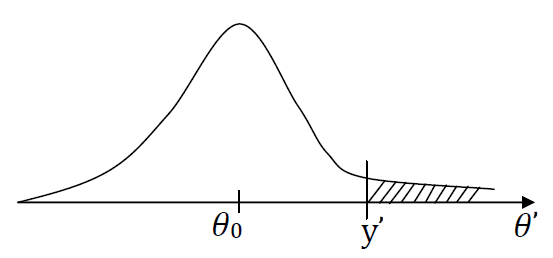
\includegraphics[scale=0.7]{Figures/Lecture8_Fig1}
\caption{1-D Location testing with Gaussian error using Composite Hypothesis Testing }
\label{1-DLocationtestCHT}
\end{figure}





\end{exmp}



\begin{exmp}
\emph{1-D Location testing with Gaussian error where UMP doesn't exist:}\\
\[\forall\ \theta \in \mathbb{R}, \quad \mathbb{P}_\theta : \mathcal{N}(\theta, \sigma^2)\]
\noindent Consider the Composite Hypothesis Test:
\begin{align*}
H_0:\theta &= \theta_0 \\
H_1:\theta &\neq \theta_0 \\
\Lambda = (-\infty,\theta_0)\cup&(\theta_0,\infty)\cup\{\theta_0\}\\
\Lambda_0 = \{\theta_0\} , \ \Lambda_1 = (&-\infty, \theta_0) \cup (\theta_0, \infty)
\end{align*}



\noindent The decision region $\Gamma_1(\theta^\prime)$ of the Neyman-Pearson test for $\theta$ versus $\theta^\prime$ is given by:
\begin{equation}
    \Gamma_1(\theta^\prime)=
    \begin{cases}
    (-\infty, \theta_0 + \sigma\Phi^{-1}(\alpha)) &\quad\theta^\prime < \theta_0\\
    (\theta_0 + \sigma\Phi^{-1}(1-\alpha), \infty) &\quad\theta^\prime > \theta_0
    \end{cases}
\end{equation}


\noindent Since $\Gamma_1(\theta^\prime)$ depends on $\theta^\prime\in\Lambda_1$, we cannot find a Uniformly Most Powerful test.\\
In fact : $\forall\ \theta^\prime < \theta_0$:
\begin{equation}
P_D({\delta_{NP}}^{<},\theta^\prime)=\Phi\left(\Phi^{-1}(\alpha)-\frac{\theta^\prime-\theta_0}{\sigma}\right) \label{pdless} \\
\end{equation}
\\and $\forall\ \theta^\prime>\theta_0$: \\
\begin{equation}
P_D({\delta_{NP}}^{>},\theta^\prime)=1-\Phi\left(\Phi^{-1}(1-\alpha)-\frac{\theta^\prime-\theta_0}{\sigma}\right) \label{pdgrt}\\
\end{equation}

\begin{figure}[h]
\centering
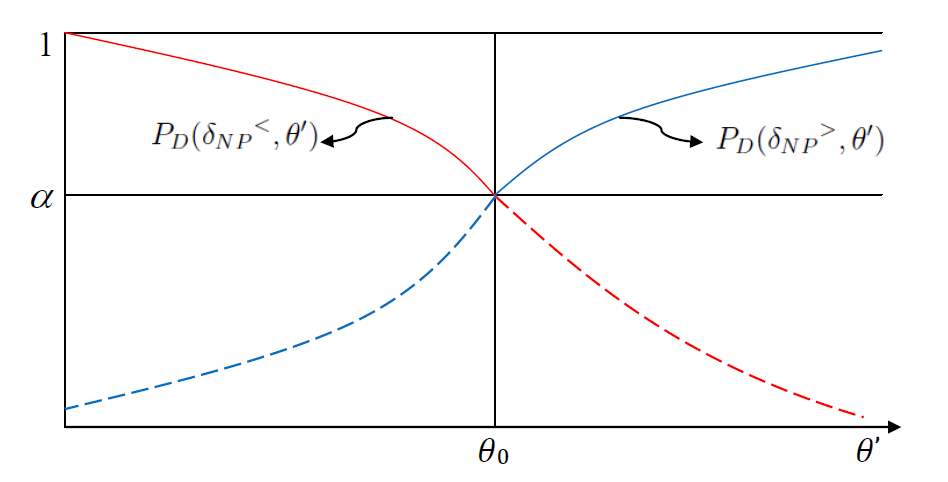
\includegraphics[scale=0.5]{Figures/Lecture8_Fig2}
\caption{Equations (\ref{pdless}) and (\ref{pdgrt}) plotted as a function of $\theta^\prime$ }
\label{UMPtestFail}
\end{figure}

\end{exmp}
\noindent Next question is can we weaken the requirement of UMP test to find a test which is powerful at most places of interest? This leads us to the next section.

\section{Locally Most Powerful (LMP) Tests}

Consider a composite hypothesis test of the form:
\begin{align*}
H_0:\theta &= \theta_0 \\
H_1:\theta &> \theta_0
\end{align*}

\noindent \emph{Goal:} We want powerful detection for $\theta\in\Lambda_1$ , near $\theta_0$.\\
Expand $P_D(\delta,\theta)$ in a Taylor series about $\theta=\theta_0$:\\
$$P_D(\delta,\theta)=P_D(\delta,\theta_0) + (\theta-\theta_0).{P_D}^\prime(\delta,\theta_0) + O((\theta-\theta_0)^2)$$\\
We would like: $P_D(\delta,\theta_0)=P_F(\delta,\theta_0)=\alpha$ , so that\\
$$P_D(\delta,\theta)\approx \alpha + (\theta-\theta_0).{P_D}^\prime(\delta,\theta_0)$$\\
Thus, maximizing $P_D(\delta,\theta)$ is equivalent to maximizing ${P_D}^\prime(\delta,\theta_0)$ since $\theta-\theta_0 \geq 0$\\

\begin{defn}
A test that maximizes ${P_D}^\prime(\delta,\theta_0)$ subject to $P_F(\delta,\theta_0) \leq \alpha$ is called an $\alpha$ - level Locally Most Powerful (LMP) test.
\end{defn}

\noindent Observe that:
\begin{align*}
{P_D}^\prime(\delta,\theta_0) &= \frac{\partial}{\partial\theta}P_D(\delta,\theta)\left| {_{\theta = \theta_0}} \right.\\ &= \frac{\partial}{\partial\theta}\mathbb{E}_\theta[\delta(y)]\left| {_{\theta = \theta_0}} \right.\\ &= \frac{\partial}{\partial\theta}\int_{\Gamma}\delta(y)p_\theta(y)dy\left| {_{\theta = \theta_0}} \right.\\ &= \int_{\Gamma}\frac{\partial}{\partial\theta}(\delta(y)p_\theta(y))\left| {_{\theta = \theta_0}} \right.dy\\ &= \int_{\Gamma}\left[\frac{\partial}{\partial\theta}p_\theta(y)\left| {_{\theta = \theta_0}} \right.\right]\delta(y)dy \\
\end{align*}

\noindent The term in square brackets in the above integrand plays the role of $p_1(y)$ from the simple Neyman-Pearson Hypothesis testing problem.
\\
Therefore, a locally most powerful test has the form:
\begin{equation}
\delta_{LMP}(y)=\begin{cases}
 1, & \frac{\partial}{\partial\theta}p_\theta(y)\left| {_{\theta = \theta_0}} \right.>\eta p_{\theta_0}(y)\\
    \gamma, & \frac{\partial}{\partial\theta}p_\theta(y)\left| {_{\theta = \theta_0}} \right.=\eta p_{\theta_0}(y)\\
    0, & \frac{\partial}{\partial\theta}p_\theta(y)\left| {_{\theta = \theta_0}} \right.<\eta p_{\theta_0}(y)
  \end{cases}
\end{equation}
where $\eta, \gamma$ are chosen such that $P_F(\delta_{LMP}, \theta_0) = \alpha$\\

\begin{rem}
Other ways of designing hypothesis tests:
\textbf{Generalized Likelihood Ratio Test (GLRT)/ Maximum Likelihood Ratio Test:}
\begin{equation}
\delta_{GLRT}(y) = \mathds{1} \left\{\frac{\underset{\theta\in\Lambda_1}{\max} p_\theta(y)}{\underset{\theta\in\Lambda_0}{\max} p_\theta(y)} \gtreqqless \eta\right\}
\end{equation}
\end{rem}

\section{Signal Detection in Discrete Time}

\noindent \emph{Goal:} Apply hypothesis testing principles to detecting signals corrupted by noise.

\subsection{Basic model of signals corrupted by noise:}
In general, the received signal is an n-dimensional vector, which can be modelled as
\[\emph{Y} \equiv {(Y_1,Y_2,\dots,Y_n)}^T \in \mathbb{R}^n\]
We can think of n as time duration of measurement.
\begin{align*}
H_0 : Y_k = S_{0k} + N_k , \quad  k \in [n]\\
H_1 : Y_k = S_{1k} + N_k , \quad  k \in [n]
\end{align*}
\noindent where $k = 1,2,\dots,n \equiv k \in [n]$
\begin{align*}
\emph{S_0} &\equiv {(S_{01},S_{02},\dots,S_{0n})}^T\\
\emph{S_1} &\equiv {(S_{11},S_{12},\dots,S_{1n})}^T\\
\emph{N} &\equiv {(N_1,N_2,\dots,N_n)}^T
\end{align*}
\noindent where $\emph{S_0}$ and $\emph{S_1}$ are signals and $\emph{N}$ is noise.\\

\Tree[.\text{Typically, $\emph{N}$ is independent of $\emph{S_0}$ and $\emph{S_1}$}  [.\text{I)$\emph{S_0}$ and $\emph{S_1}$ are } ]
               [.\text{II)$\emph{S_0}$ and $\emph{S_1}$ are partially } ] 
               [.\text{III) $\emph{S_0}$ and $\emph{S_1}$ are } ]]\\
\indent \hspace{1cm} deterministic and known \quad \quad deterministic and \hspace{1cm} completely random\\
\indent \hspace{6cm} partially random

\end{document}